\chapter{Experimental Results\label{chap:exp}}

The overhead introduced by oxc framework composes three parts:
\begin{itemize}
\item The time required to execute codes brought oxc functions.
\item The context switches introduced by the oxc framework.
\item The degradation of modular schedulers' performance under oxc 
	framework.
\end{itemize}

The third item is caused by implementation skills and not the emphasis
of our experiments. For example, the per CPU runqueue is a per CPU 
structure, which can be more efficiently accessed than per ox container 
runqueue. However, such a difference can be solved with efforts on 
implementation details. 

There are two experiments carried out to evaluate the overhead in the oxc
framework. In experiment A, the codes execution
time of frequently invoked oxc functions is measured. In experiment B, the
overall overhead of oxc control is estimated through comparisons with rt 
throttling and cfs bandwidth control.

Inside each oxc function, there is a scheduling operation encapsulated and
extra codes to control bandwidth reservation. The execution time of these
control codes is the main interest in experiment A.
Current oxc framework implementation is still a prototype one. Some kernel 
features are not considered under the framework yet. For example, the 
\texttt{priority inheritance}, which is important for the kernel's real time
performance and will influence number of context switches. So the overhead
result in experiment B in shown in a relative way instead of precisely 
statistical analysis. As for the context switches caused by importng CBS 
based scheduling in the kernel, there is previous work in \cite{Luigi09};
yet these results do not straightly apply to oxc work. 

The hardware and software used in the experiment is shown in 
table \ref{tab:exp_setup}.
\begin{table}[H]%thbp]
  \centering
  \begin{tabular}{ll}\hline
	\emph{Hardware platform}\hspace{4cm}		& 	\\
	Processor			& Intel(R) Core(TM) Duo E8500	 \\
	Frequency			& 3.16GHz\\
	RAM				& 	  \\	
					&	\\	
	\emph{Software platform}\hspace{4cm}		& 	\\
	Linux distribution		& Ubuntu 11.10\\
	Compiler version		& gcc 4.6.1\\
	Kernel version			& 3.4.0-rc+ \\\hline
  \end{tabular}
  \caption{Hardware-Software platform}
  \label{tab:exp_setup}
\end{table}
This chapter is organized like this: the tracing tool and synthetic benchmark
tool we use in the experiment are described; then it's the design of each 
experiment and result analysis; finally, what we learn from the experiment
is concluded.

\section{Ftrace in Linux kernel}
Ftrace\cite{ftrace} is an internal tracer designed to help out developers of systems to
find out what is going on inside the kernel. The name ftrace comes from
''function tracer'', which is its original purpose and the reason it is 
used here. Now there are various kinds of tracers incorporated in Ftrace.
You can use it to trace context switces, hong long interrupts are disabled,
and so on.

Ftrace uses \emph{debugfs} file system to hold control files as well as
file to display output. 
Typically, ftrace is mounted at \texttt{/sys/kernel/debug}.
\begin{lstlisting}
	#mount -t debugfs nodev /sys/kernel/debug
\end{lstlisting}
After this command, a firectory \texttt{/sys/kernel/debug/tracing} will 
be created containing interfaces to configure ftrace and display results.
\begin{lstlisting}
	#cd /sys/kernel/debug/tracing
\end{lstlisting}
The following commands will be assumed to be called under \texttt{tracing}
directory.
There are several kinds of tracers available in ftrace, simply cat the
\texttt{available\_tracers} file in the \texttt{tracing} dorectory.
\begin{lstlisting}
	#cat available_tracers
	blk function_graph mmiotrace wakeup_rt wakeup function sched_switch nop
\end{lstlisting}
The \texttt{function} is function tracer. It uses the \texttt{-pg} option
of \texttt{gcc} to have every function in the kernel call a special function
\texttt{mcount()} for tracing all kernel functions and measure execution time 
of them.  This is what we need. To enable the function tracer, just \emph{echo} \texttt{function} into the \texttt{current\_tracer}
file.
\begin{lstlisting}
	#echo function > current_tracer
\end{lstlisting}
The trace can be started and stopped through configuring \texttt{tracing\_on}
file. Echo 0 into this file to disable the tracer or 1 to enable it. Cat the
file will displat whether the tracer is enabled or not.

The output of the trace in held in file \texttt{trace} in a human readable
format. The ftrace will by default trace all functions in the kernel. In
most cases, people only care about particular functions. To dynamically
configure which function to trace, the \texttt{CONFIG\_DYNAMIC\_FTRACE}
kernel option should be set in compilation time  to enable dynamic ftrace. 
Actually, \texttt{CONFIG\_DYNAMIC\_FTRACE} is highly recommanded and defaultly
set because of its performance enhancement. To filter which function to trace
or not, two files are used, one for enabling and one for disabling the 
tracing of specific functions. They are \texttt{set\_ftrace\_filter} and 
\texttt{set\_ftrace\_notrace}. A list of available functions that you can add
to these files is listed in \texttt{available\_filter\_functions}.

\section{Tbench}
The tbench benchmark is a tool that measures disk throughput for simulated
netbench run. Tbench reads a load description file called client.txt that was
derived from a network sniffer dump of a real netbench run and produces the
filesystem load according to the description file. It produces only the TCP
and process load and no filesystem calls.
One exmple to run tbench test:
\begin{lstlisting}
	$tbench_srv
	$tbench 2 -t 100
\end{lstlisting}
The \texttt{tbench\_srv} should be invoked before running \texttt{tbench}.
The second starts two tbench connections with one client and one server in
each connection. The two connections will run simultaneously and the runtime
of the benchmark will be 100 seconds.

\section{Experiment A}
\subsection{The experiment design}
In this experiment, the execution time of oxc functions are measured.
In a Linux system, even if the oxc patch is applied in the kernel, when 
there is no reservation enabled, the system performs as a plain Linux system. 
The possible oxc overheads in this case include the code execution time in 
function \texttt{is\_oxc\_task} and the oxc related initialization when a 
scheduling group is created; both are negligible.

During the experiment, the execution time of following oxc functions are 
measured using Ftrace:
\begin{itemize} 
\item \texttt{check\_preempt\_curr\_oxc}
\item \texttt{pick\_next\_task\_oxc}
\item \texttt{put\_prev\_task\_oxc}
\item \texttt{task\_tick\_oxc}
\end{itemize} 
They are most often called oxc functions as they enclose in most frequently
invoked scheduling operations. The oxc functions like 
\texttt{enqueue\_task\_rq\_oxc} and \texttt{dequeue\_task\_rq\_oxc} only 
happen when a task enters or leaves an ox container. Inside an
ox container, enqueue and dequeue of a task still frequently happen.
However, the performance of scheduling operations of each modular
scheduler under oxc framework is not an interest in this experiment.


There will be six individual tests differing in the number of
hyper ox containers in the system. The number of hyper ox containers in
different will vary from 1 to 6.
The hyper ox containers in the experiment are identical.
Each hyper ox-container has two ox containers with the same CPU reservation 
parameter $0.1ms/1ms$. Each ox container has one dummy task within it. 
The dummy task is simply running a forever while loop and it is a rt task with 
policy \texttt{SCHED\_FIFO}. This while loop task will exhuaust the 
reservation in an ox container. The scheduling policy is arbitrarily chosen 
without special thoughts.

The measured execution time of above oxc functions comprises the time 
consumed by codes involving with the oxc control and operations defined 
in modular scheduler which are encapsulated inside the above functions.
Here the situation for rt scheduling inside an ox container is very simple.
And the experiment analysis can focus on oxc control overhead.

\subsection{Experiment results}
The statistics results of six tests are listed in table \ref{tab:exp_res}.
The index of a text is the number of hyper ox containers in that test.
The two fields in the pair are average time and standard deviation of the
function execution and are measured in micro seconds.
\begin{table}[thbp]
	\centering
	\begin{tabular}{|l||c|c|c|c|c|c|}\hline
		& \tiny{test1} & \tiny{test2} & \tiny{test3} & \tiny{test4} & \tiny{test5} & \tiny{test6}\\\hline
	\tiny{pick\_next\_task\_oxc} &\tiny{(0.168, 0.083)} &\tiny{(0.155, 0.070)} &\tiny{(0.206, 0.178)} 
							&\tiny{(0.230, 0.215)} &\tiny{(0.211, 0.216)} & \tiny{(0.246, 0.251)} \\\hline
	\tiny{put\_prev\_task\_oxc} &\tiny{(0.827, 0.049)} & \tiny{(0.834, 0.096)}&\tiny{(0.820, 0.103)} &\tiny{(0.801, 0.111)} &
					\tiny{(0.829, 0.146)} & \tiny{(0.852, 0.251)}\\\hline
	\tiny{task\_tick\_oxc} &\tiny{(0.272, 0.192)} & \tiny{(0.275, 0.182)}&\tiny{(0.263, 0.155)} & \tiny{(0.261,0.15)}& \tiny{(0.245,0.158)}& 
					\tiny{(0.249,0.146)}\\\hline
	\tiny{check\_preempt\_curr\_oxc} & - & - & - & - & - & - \\\hline
	\end{tabular}
	\caption{Measured execution time, in micro seconds, of oxc functions\\
				 \indent\hspace{4cm}in the format of \emph{(mean, standard deviation)}}
	\label{tab:exp_res}
\end{table}

The first observation is from the row for 
\texttt{check\_preempt\_curr\_oxc}. That is, no tracing result for 
\texttt{check\_preempt\_curr\_oxc} is recorded.
An analysis of overhead in this function is necessary.
There are three cases for the comparison between a task and currently 
the running task. When only one of them is an oxc
task or both two are oxc tasks and not in the same containers, the comparison 
cost is just several \texttt{if-else} instructions. If they are two oxc tasks
in the same container, the comparison follows the procedure in Linux scheduling
and this is not overhead from oxc control; in addition, in our experiment 
setup, there is only one task inside an ox container.
In one statement, this function is not a big soure for oxc control overhead. 
Although this could be a reason to explain that the ftrace fails to measure
the execution time of \texttt{check\_preempt\_cur\_oxc} during tests, it reminds
us that, given the feature of hierarchical scheduling, it may be attractive to
develop a new recording tool so as to evaluate the oxc framework more accurately.
 
The test results of other three oxc functions are illustrated in figure 
\ref{fig:pick_next}, \ref{fig:put_prev} and \ref{fig:task_tick}.
The variable parameter in each test is the number of ox containers.
And experimental results show that at least in current oxc framework, the
codes execution time are influenced by the number of containers in the
system.
\begin{figure}[htbp]
        \centering
        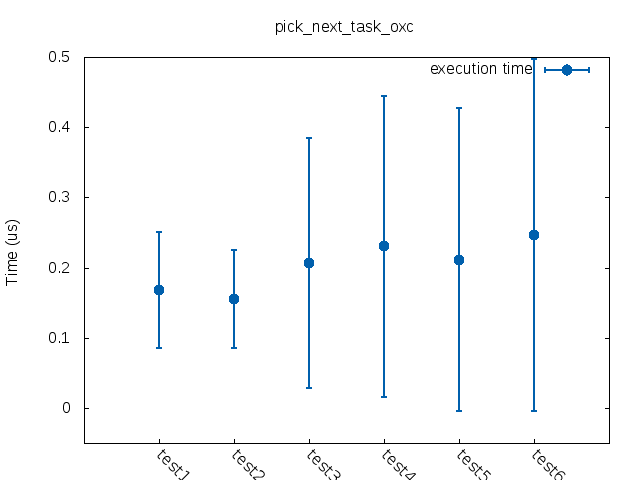
\includegraphics[width=\textwidth]{images/pick_next_task_oxc}
        \caption{Experiment results for \texttt{pick\_next\_task\_oxc}}
        \label{fig:pick_next}
\end{figure}
\begin{figure}[htbp]
        \centering
        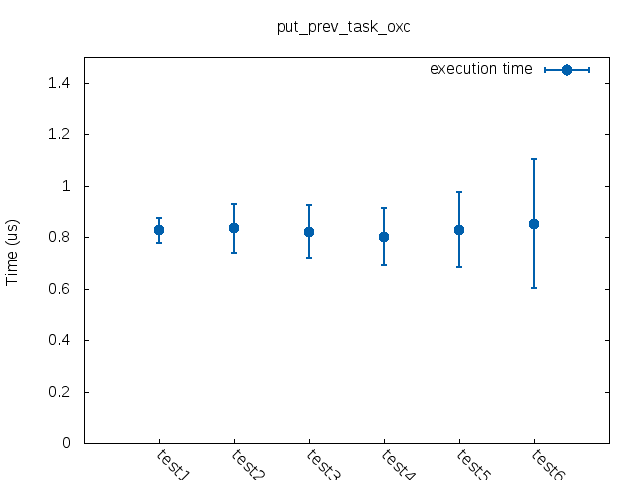
\includegraphics[width=\textwidth]{images/put_prev_task_oxc}
        \caption{Measured execution time for \texttt{put\_prev\_task\_oxc}}
        \label{fig:put_prev}
\end{figure}
\begin{figure}[htbp]
        \centering
        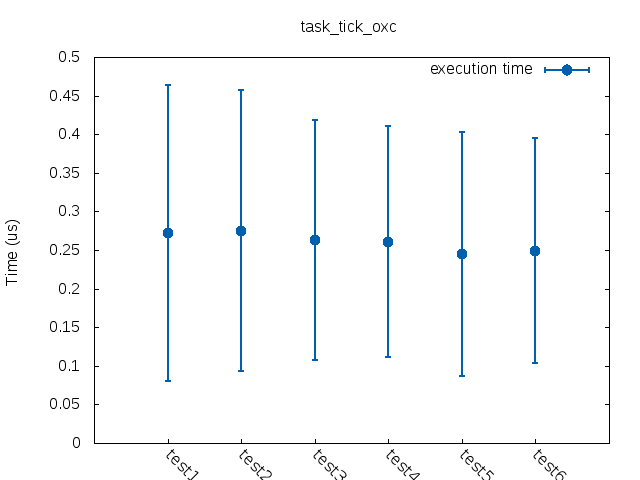
\includegraphics[width=\textwidth]{images/task_tick_oxc}
        \caption{Experiment results for \texttt{task\_tick\_oxc}}
        \label{fig:task_tick}
\end{figure}
Figure \ref{fig:pick_next} shows the statistical result of 
\texttt{pick\_next\_task\_oxc} in each test. One observation from the figure
is that with more ox containers joining the system, the time spent on executing
the function codes fluctuates more. This trend also reflects in the
results for \texttt{put\_prev\_task\_oxc}, shown in figure \ref{fig:put_prev}.
However, figure \ref{fig:task_tick} for \texttt{task\_tick\_oxc} does not 
show this pattern.

Actually, the oxc control codes in the three oxc functions are the same:
to update the per CPU runqueue, to update the per container runqueue and
update the current ox container. So the different variance behaviours in
results for tested oxc functions are caused by the scheduler's performance
under inside a container. More specifically, the difference in accessing 
per CPU and per ox container runqueue could be the reason for variance 
changing trend. 

The \texttt{task\_tick\_oxc} encloses in the \texttt{task\_tick} scheduling
operation. In our experiment, it is \texttt{task\_tick\_rt}. A look at 
the content inside this method in list \ref{task_tick_rt}. Compare it 
with the other two tested oxc functions' content, it's operations with
runqueue is very simple. This explains why the result in \ref{fig:task_tick}
is stable in both mean value and standard variance.
\begin{lstlisting}[language=C,
			caption={\texttt{task\_tick\_rt}},
			label={task_tick_rt}]
static void task_tick_rt(struct rq *rq, struct task_struct *p, int queued)
{
        update_curr_rt(rq);

        watchdog(rq, p);

        /*
         * RR tasks need a special form of timeslice management.
         * FIFO tasks have no timeslices.
         */
        if (p->policy != SCHED_RR)
                return;
	/*
         * The left part has no effects in our tests.
	 */
	...

}
\end{lstlisting}



\section{Experiment B}
\subsection{Experiment design}
The aim of this experiment is to estimate the overall overhead in oxc 
framework through non real-time CPU bandwidth control mechanisms that 
are already in Linux kernel.
During tests the synthetic load is generated by the tbench benchmark tool.
The CPU bandwidth allocated to tbench connections are allocated by oxc 
control, rt throttling and cfs bandwidth control individually. 
The tbench throughput results of oxc framework are then compared with 
rt throttling and cfs bandwidth control. Through such comparisons, the 
overhead introduced by oxc control is then evaluated in a relative way.

Two \emph{tbench} connections will be set up in the system.
Each connection will be dedicated to one CPU.
Without constraints, they will consume all CPU time.
In the experiment, the CPU bandwidth allocated to tbench traffic is restricted.
The tested per CPU bandwidth parameter includes
$0.05ms/1ms$, $0.1ms/1ms$, $0.2ms/1ms$, $0.4ms/1ms$, $0.6ms/1ms$ and 
$0.8ms/1ms$. 
Again, this is per CPU bandwidth that is planned to assign to \emph{tbench}
tasks. Each cpu bandwidth control mechnism will restricts the \emph{tbench}
execution not exceed the configured value. And the throughput results will
reflect the overhead in three work through a relative way.

When rt throttling is tested, \emph{tbench} clients and servers will be 
scheduled as rt tasks with policy \texttt{SCHED\_RR}. Otherwise the client 
and server in the same connection cannot run at all. Correspondingly, when 
comparing with rt throttling, \emph{tbench} threads inside containers will 
be set as rt tasks with \texttt{SCHED\_RR} policy. 
When comparing the oxc control with cfs bandwidth control, the \emph{tbench}
threads will be put inside two ox containers and they will run as normal
tasks. 

\subsection{Experiment results}
The test results are shown in table \ref{tab:expB1} and \ref{tab:expB2}.
\begin{table}[thbp]
	\centering
	\begin{tabular}{|l||c|c|}\hline
		 per CPU bandwidth & rt throttling & oxc control + rt scheduling\\\hline
			0.05/1ms &	21.9335	&	18.5313	\\\hline 
			0.1ms/1ms &	43.5794 &	36.89324 \\\hline
			0.2ms/1ms &	92.7356 &	73.5099	\\\hline
			0.4ms/1ms &	172.582 &	147.806 \\\hline
			0.6ms/1ms &	233	&	225.72	\\\hline
			0.8ms/1ms &	319.297 &	297.0607	\\\hline
	\end{tabular}
	\caption{Measured throughput, in Mbps/sec, between rt throttling and oxc control}
	\label{tab:expB1}
\end{table}
\begin{table}[thbp]
	\centering
	\begin{tabular}{|l||c|c|}\hline
		 per CPU bandwidth & cfs bandwidth control & oxc control + cfs scheduling  \\\hline
		 0.05ms/1ms	& 24.8825	& 19.2151 \\\hline
		 0.1ms/1ms	& 52.2106	& 39.4268 \\\hline
		 0.2ms/1ms	& 106.226	& 77.4225 \\\hline
		 0.4ms/1ms	& 215.071	& 151.465 \\\hline
		 0.6ms/1ms	& 323.628	& 234.369 \\\hline
		 0.8ms/1ms	& 433.025	& 305.1 \\\hline
	\end{tabular}
	\caption{Measured throughput, in Mbps/sec, between cfs bandwidth and oxc control}
	\label{tab:expB2}
\end{table}
A glance on the two tables, it's apparantly to see that the throughput results
under cfs bandwidth control outperforms the other two. There are two reasons for this.
Firstly, the overhead brought by cfs bandwidth control is indeed lower 
than the other two bandwidth control mechnanisms.
And both oxc tasks and rt tasks are more greedy than cfs tasks when they occupy a CPU. 
An oxc task or rt tasks will not give up a CPU to a cfs task until the 
CPU reservation is all consumed and most tasks in Linux are scheduled by cfs.
So the system is stressed more under oxc control or rt throttling.
However, in cfs scheduling, cfs tasks, with or without
CPU reservation, can share the CPU evenly.

Having solved the above question, let's see the overhead in oxc framework.
In figuer \ref{fig:expB1}, the throughput results in different reservation
parameters under oxc control and rt throttling are shown.
At first, the throughput result under rt throttling is growing faster 
than the result in oxc control. However, as the more CPU bandwdith is
reserved to tbench tasks, the throughtput of the two are converging.
In fact, the throughtput growing trend in oxc control are consistent.
When it comes to rt throttling, it's not like this.
When a relatively small fraction of CPU is assigned to rt throttling
and oxc control, rt throttling shows better performance. However, with
increasing the reserved CPU bandwdith, the stress of rt throttling on
the whole system is increasing too, which slows the throughput growing. 
The performance in oxc control is interesting. The increasement of 
throughput result is almost linear with the change of reserved bandwidth.
The overhead in oxc control is almost a constant value.

The comparason between oxc control and CPU bandwidth control is ahown 
in figure \ref{fig:expB2}. As we just analyzed, cfs bandwidth control has
much better throughput result. One observation is that althouth with
less rasing speed, the throughput increasing trend in oxc control has the
similar shape as in cfs bandwidth control. 

There is another meaningful comparasons shown in figure \ref{fig:expB3}, which
is the throughtput results of rt scheduling and cfs scheduling under oxc 
framework. The results are quite close, and the difference can be regarded as
the scheduling cose between rt and cfs scheduling in an ox container.

\begin{figure}[htbp]
        \centering
        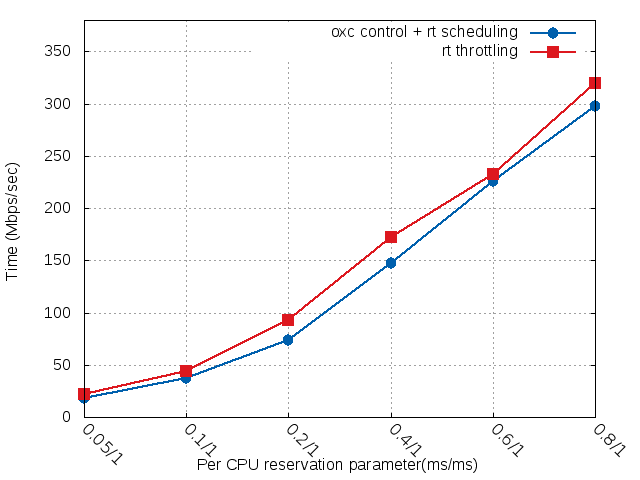
\includegraphics[width=\textwidth]{images/expB1}
        \caption{\emph{oxc control} vs. \emph{rt throttling}}
        \label{fig:expB1}
\end{figure}
\begin{figure}[htbp]
        \centering
        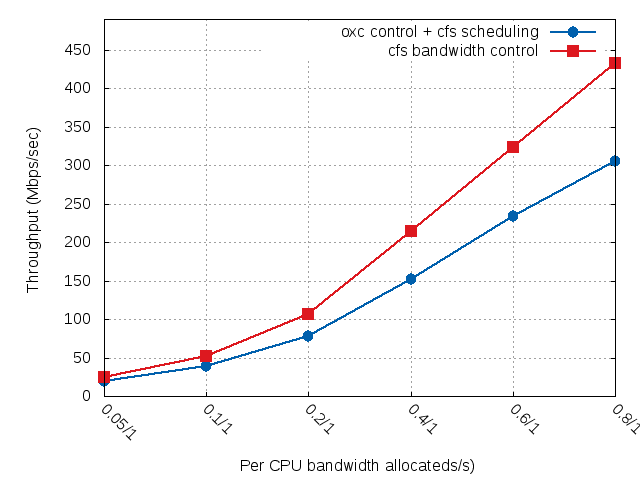
\includegraphics[width=\textwidth]{images/expB2}
        \caption{\emph{oxc control} vs. \emph{cfs bandwidth control}}
        \label{fig:expB2}
\end{figure}
\begin{figure}[htbp]
        \centering
        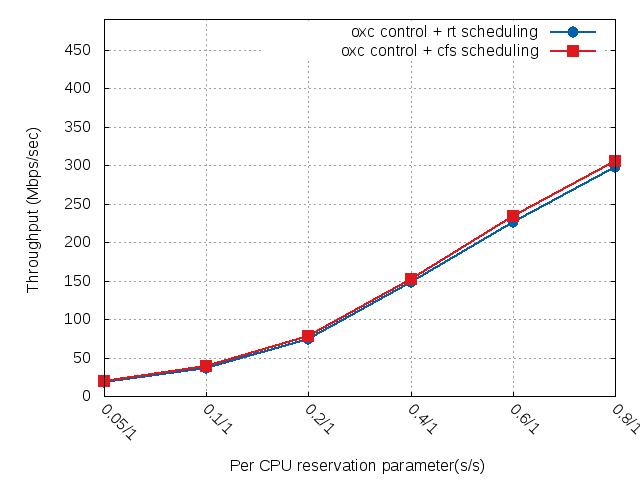
\includegraphics[width=\textwidth]{images/expB3}
        \caption{\emph{oxc control + rt throttling} vs. \emph{oxc control + cfs scheduling}}
        \label{fig:expB3}
\end{figure}
\subsection{What learnt from the experiment}
